\begin{figure}[ht!]
	\centering
	\begin{tabular}{cc}
		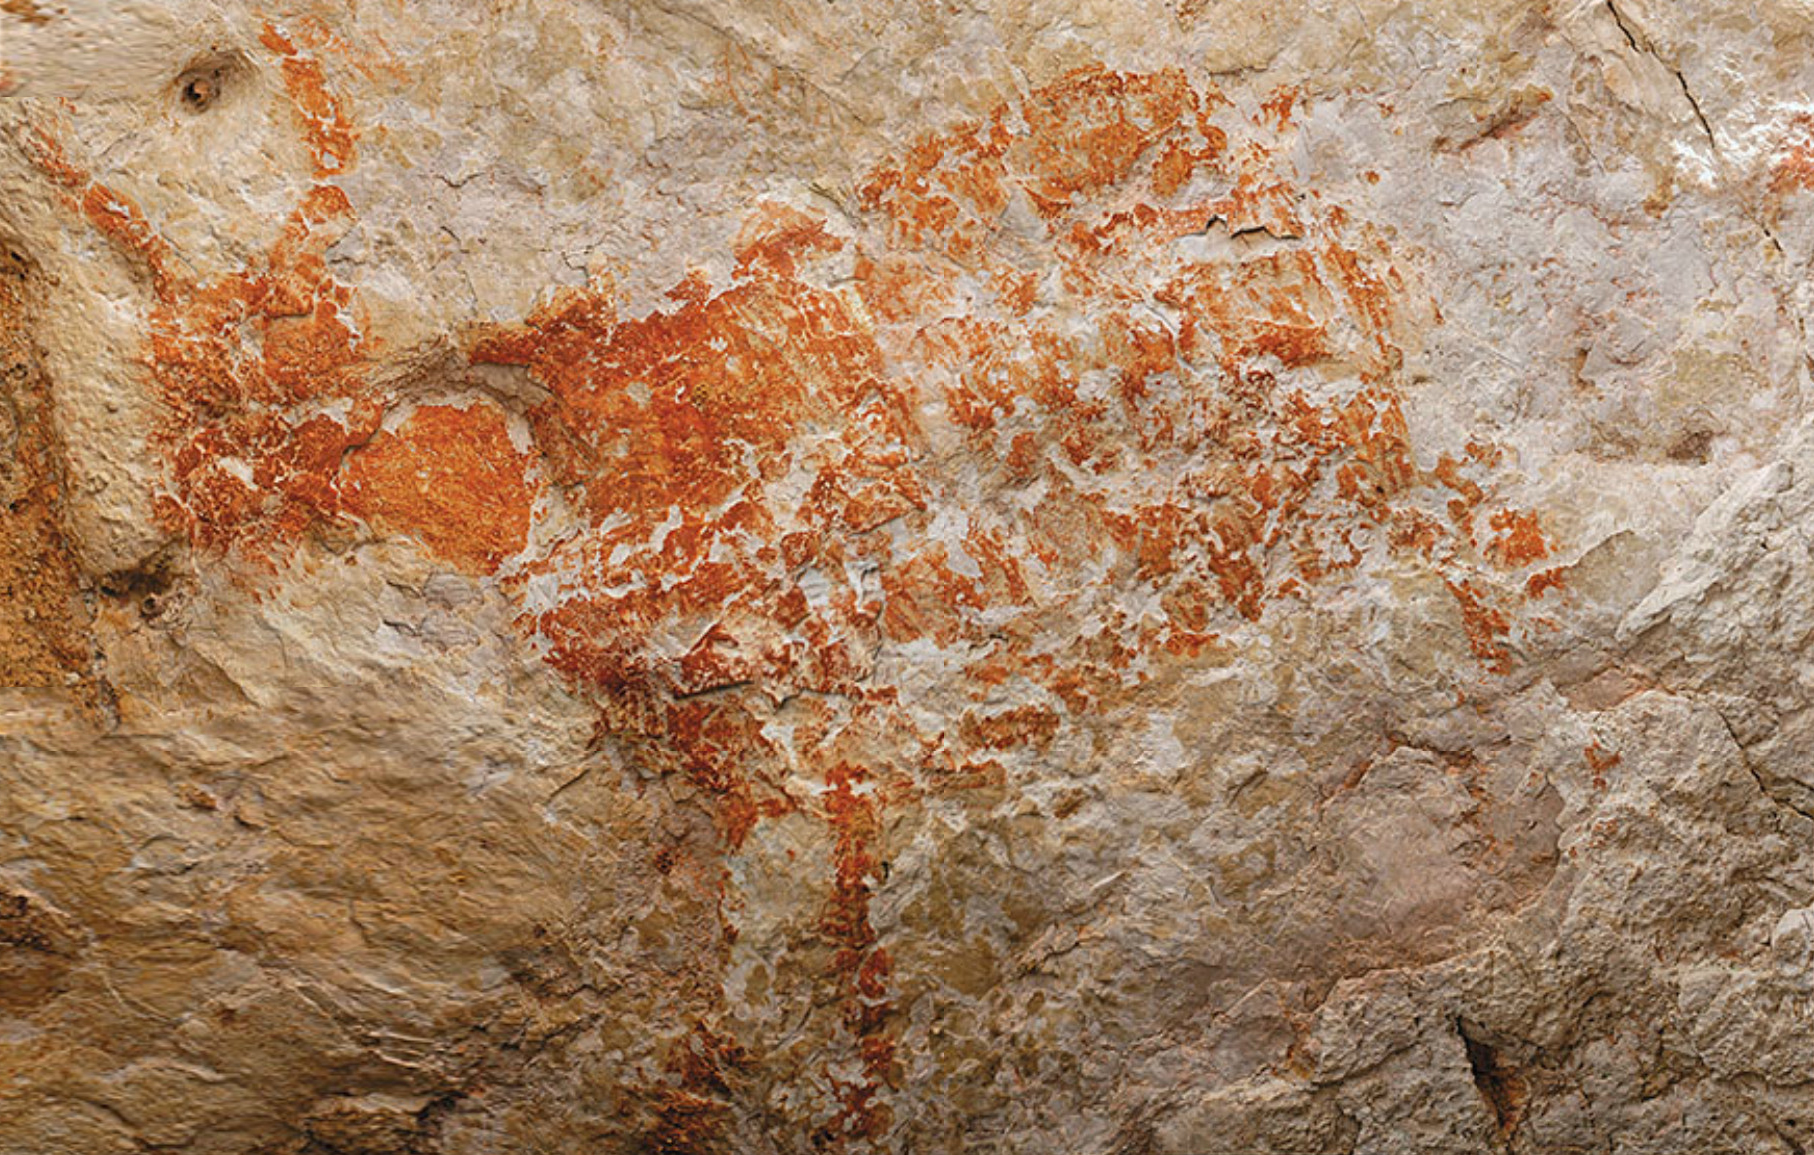
\includegraphics[width=0.49\linewidth]{figures/intro/cave_painting_of_bull.jpeg} &
		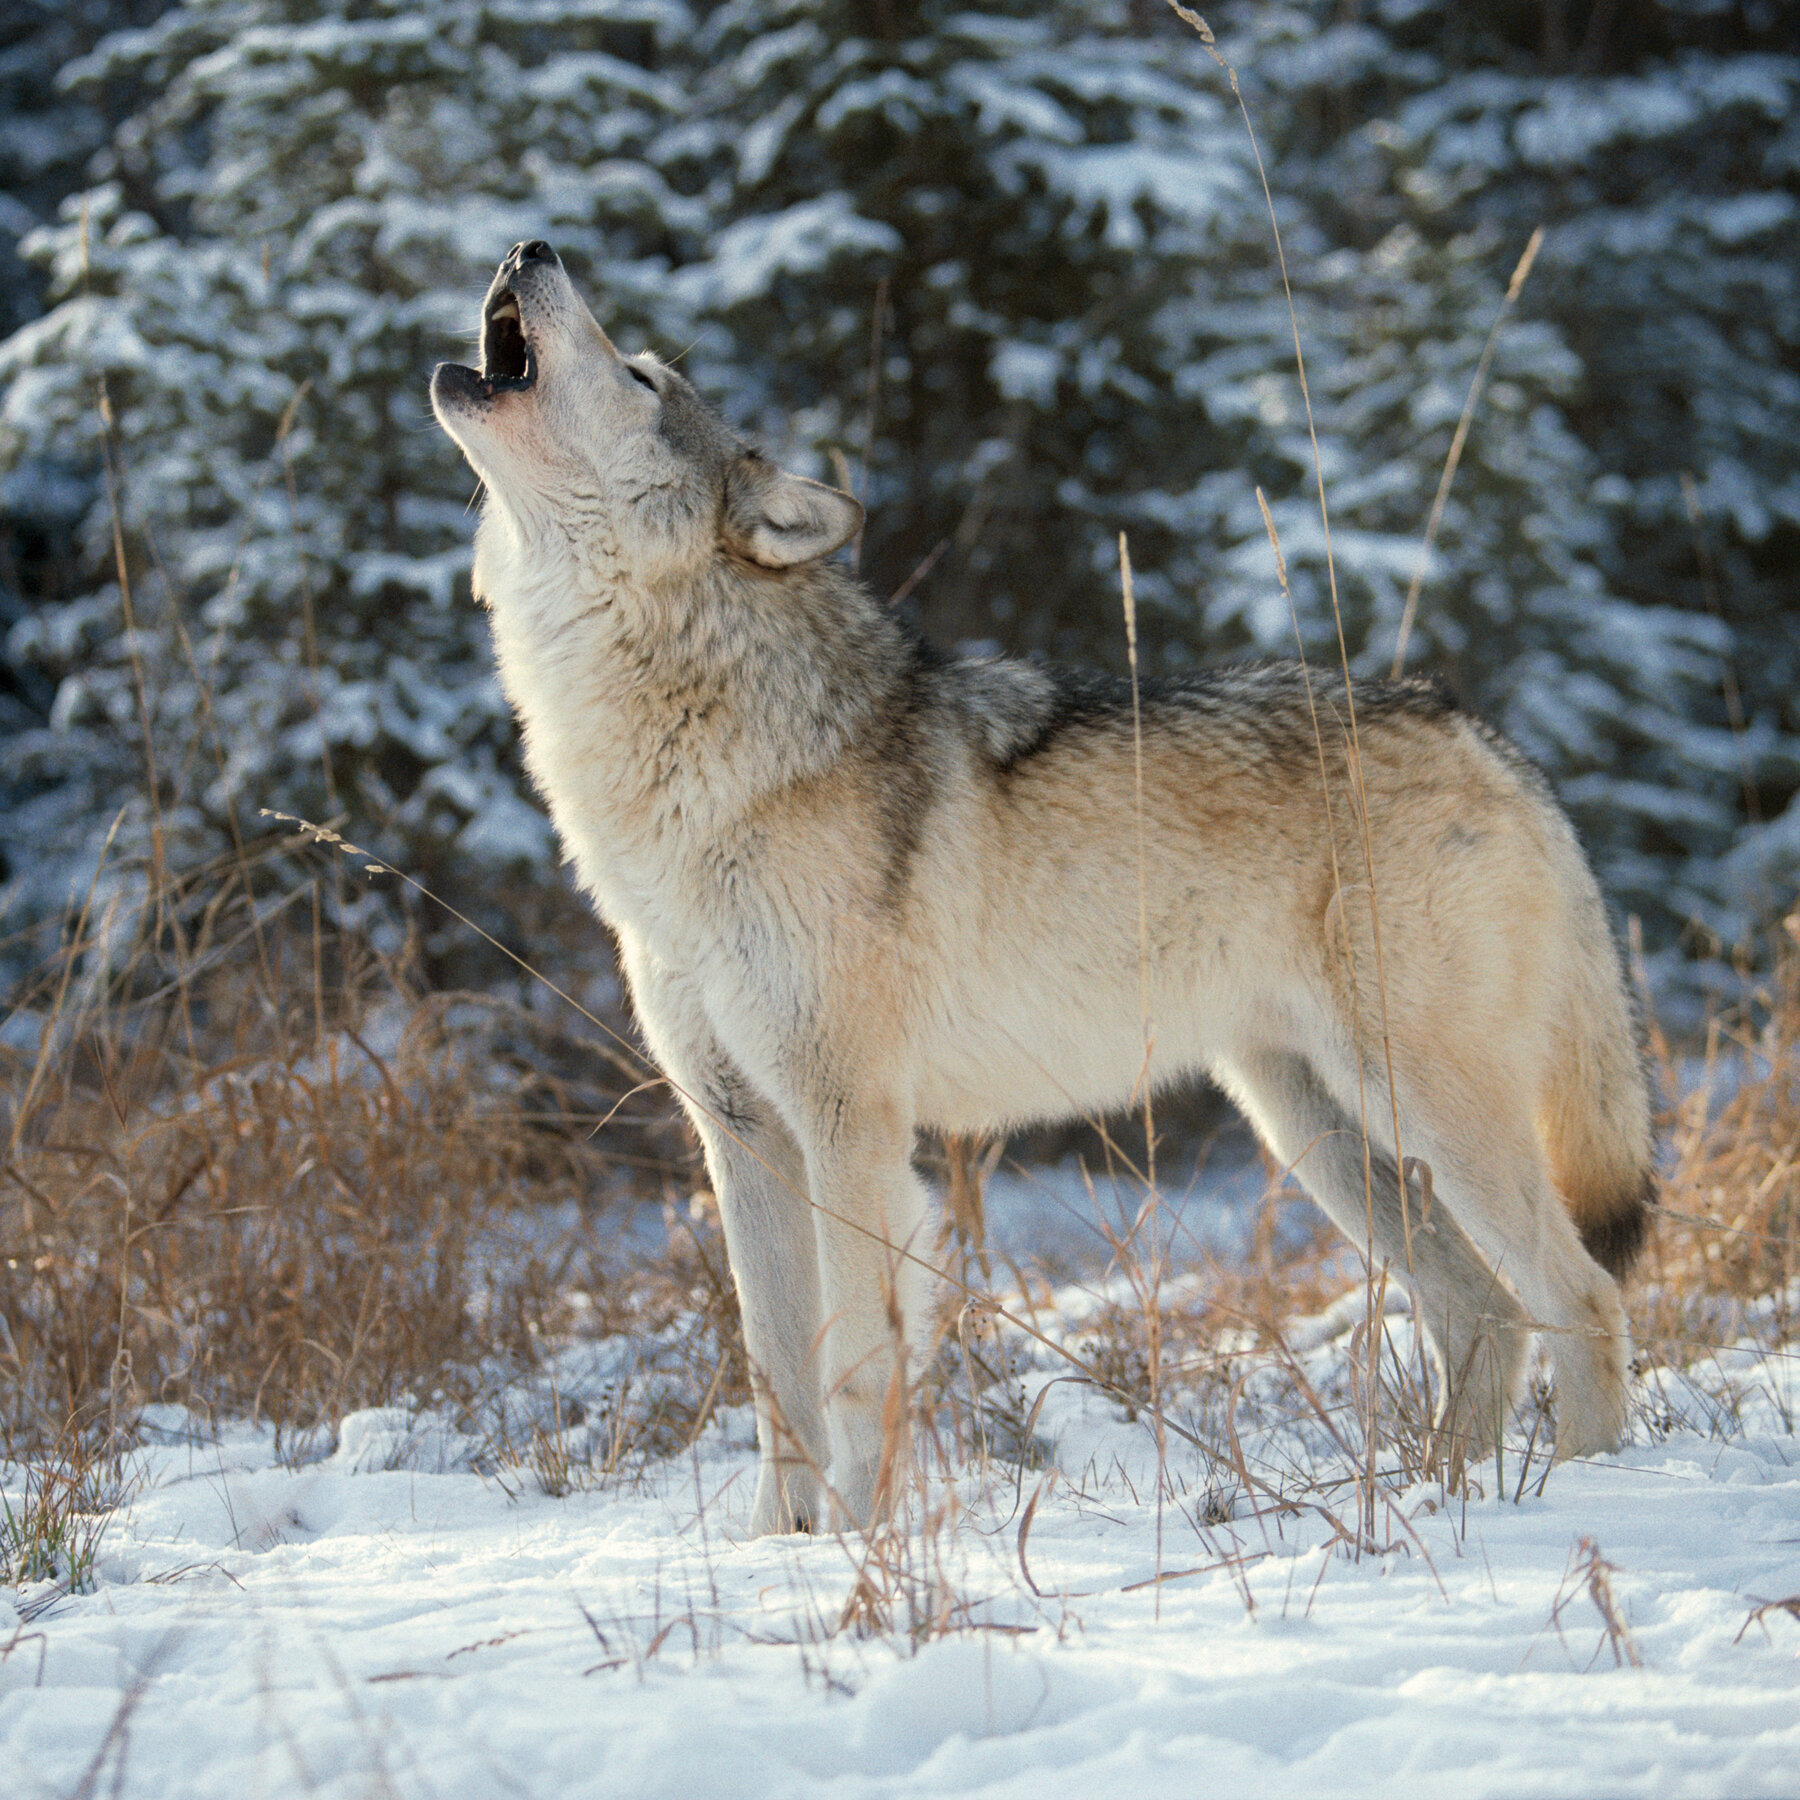
\includegraphics[width=0.31\linewidth]{figures/intro/wolf_nyt.jpeg}
		\\
	%(a) One of the oldest known figurative paintings, a depiction of an unknown bovine, was discovered in the Lubang Jeriji Saléh cave and dated to be more than 40,000 (perhaps as old as 52,000) years old. & (b) Recent photograph of a wolf from New York Times
	\end{tabular}	
	\caption[Efficacy of visual communication]{
		We are able to recognize the bovine creature almost as succinctly as we understand the wolf. However if we're magically transported to the past when this was being painted we wouldn't understand any of the language being spoken.
		}
	\label{fig:cave_painting}
\end{figure}